\chapter[Эксплуатация]{Эксплуатация \cg{} в поле}
\label{chap:operating_the_cg6_autograv_in_the_field}

Теперь вы познакомились с прибором \cg{} и правильно настроили его конфигурацию
для предстоящего исследования.

В этой главе рассматриваются основные этапы, которые необходимо выполнить при
проведении съёмки. Вот эти этапы:
\begin{itemize}
  \item Назначение пункта наблюдения с представлением в стандартном стиле

  \item Назначение пункта наблюдения с представлением в цифровом стиле

  \item Введение информации о местоположении при помощи встроенного блока GPS

  \item Выполнение измерения при помощи прибора \cg{}

  \item Регистрация данных, собранных с помощью прибора \cg{}

  \item Просмотр данных, собранных с помощью прибора \cg{}

  \item Обращение к данным, собранным с помощью прибора \cg{}
\end{itemize}

\section[Назначение пункта]{Назначение пункта наблюдения с представлением в стандартном стиле}

\infobox{
  Обратитесь к предыдущей главе, где описывается, как выбрать стандартный стиль
  представления.
}


\subsection{Использование кнопок <<+/\textminus{}>>}

\begin{figure}[h]
  \centering
  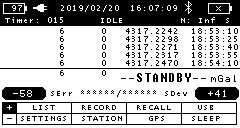
\includegraphics[width=0.49\textwidth]{figures/+_-_buttons_under_standard_station_style_1}
  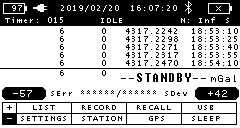
\includegraphics[width=0.49\textwidth]{figures/+_-_buttons_under_standard_station_style_2}
  \caption{Кнопки <<+/\textminus{}>> в режиме стандартного представления}
  \label{fig:+_-_buttons_under_standard_station_style}
\end{figure}

При помощи кнопок + и \textminus{}, расположенных в левой части экранного
изображения, вы можете просмотреть пункты наблюдения в предварительно
составленном списке. Чтобы просмотреть пункты наблюдения в списке, при помощи
кнопок управления наведите курсор на поле + или на поле \textminus{}, после чего
нажмите кнопку \textbf{Enter}.

\subsection{Выбор из предварительно составленного списка пунктов наблюдения}

В главном экранном изображении наведите курсор на пункт \textbf{LIST}
(изображение внизу слева) и нажмите кнопку \textbf{Enter}. Откроется экран,
показанный справа:

\begin{figure}[h]
  \centering
  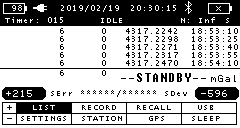
\includegraphics[width=0.49\textwidth]{figures/station_list_screen_1}
  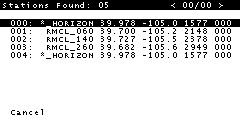
\includegraphics[width=0.49\textwidth]{figures/station_list_screen_2}
  \caption{Экран со списком пунктов наблюдения}
  \label{fig:station_list_screen}
\end{figure}

Чтобы выбрать нужный пункт наблюдения, наведите на него курсор и нажмите кнопку
\textbf{Enter}. После этого вы вернётесь в главное экранное изображение
измерения.

Чтобы покинуть это экранное изображение без изменений:
\begin{itemize}
  \item наведите курсор на пункт \textbf{CANCEL}, после чего нажмите кнопку
    \textbf{Enter}, или

  \item нажмите кнопку \textbf{Back} или \textbf{Home}.
\end{itemize}

\infobox{
  Предварительно составленный список пунктов наблюдения хранится в файле
  <<\textbf{stations.txt}>>, в корневой папке гравиметра \cg{}. Для внесения
  изменений в список обратитесь к указаниям под заголовком
  \nameref{sec:setting_up_the_pre-set_list_of_stations} в предыдущем разделе.
}

\infobox{
  Предварительно составленный список пунктов наблюдения доступен только в режиме
  стандартного стиля представления пунктов наблюдения. Режим цифрового
  представления пунктов наблюдения позволяет просмотреть список, но выделение
  сделать невозможно.
}

\subsection{Введение информации о пунктах наблюдения вручную}

На главном экранном изображении наведите курсор на пункт \textbf{STATION}
(изображение внизу слева) и нажмите кнопку \textbf{Enter}. Откроется экран,
показанный справа:

\begin{figure}[h]
  \centering
  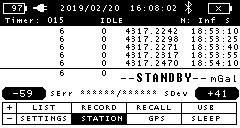
\includegraphics[width=0.49\textwidth]{figures/station_screen_under_standard_station_style_1}
  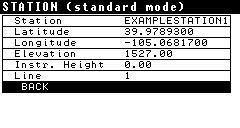
\includegraphics[width=0.49\textwidth]{figures/station_screen_under_standard_station_style_2}
  \caption{Экран пунктов наблюдения в стандартном стиле}
  \label{fig:station_screen_under_standard_station_style}
\end{figure}

На этом экранном изображении вы можете вручную ввести название пункта
наблюдения, широту, долготу, высоту над у/моря, и высоту прибора, которая
используется для введения поправки на свободный воздух на этапе обработки, а
также номер профиля.

\section[Назначение пункта]{Назначение пункта наблюдения в цифровом стиле}

\infobox{
  Обратитесь к предыдущей главе, где описывается, как выбрать цифровой стиль
  представления и величину шага приращения.
}

\subsection{Использование кнопок <<+/->>}

\begin{figure}[h]
  \centering
  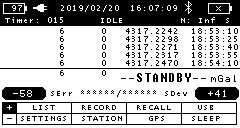
\includegraphics[width=0.49\textwidth]{figures/+_-_buttons_in_numeric_mode_1}
  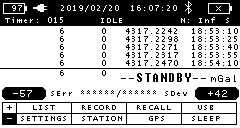
\includegraphics[width=0.49\textwidth]{figures/+_-_buttons_in_numeric_mode_2}
  \caption{Кнопки <<+/\textminus{}>> в режиме цифрового представления}
  \label{fig:+_-_buttons_in_numeric_mode}
\end{figure}

Вы можете увеличивать или уменьшать номер вашего пункта наблюдения, используя
кнопки + и \textminus{} в левой части экранного изображения. Чтобы увеличить или
уменьшить номер вашего пункта наблюдения, при помощи \textbf{кнопок управления}
наведите курсор на поле + или на поле \textminus{}, после чего нажмите кнопку
\textbf{Enter}.

\subsection{Введение информации о пунктах наблюдения вручную}

На главном экранном изображении наведите курсор на пункт \textbf{STATION}
(изображение внизу слева) и нажмите кнопку \textbf{Enter}. Откроется экран,
показанный справа:

\begin{figure}[h]
  \centering
  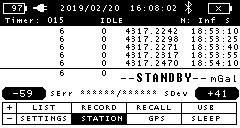
\includegraphics[width=0.49\textwidth]{figures/station_screen_in_numeric_mode_1}
  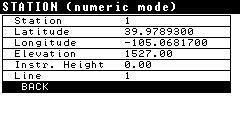
\includegraphics[width=0.49\textwidth]{figures/station_screen_in_numeric_mode_2}
  \caption{Цифровой стиль представления пунктов наблюдения}
  \label{fig:station_screen_in_numeric_mode}
\end{figure}

На этом экранном изображении вы можете вручную ввести название пункта
наблюдения, широту, долготу, высоту над у/моря, и высоту прибора, которая
используется для введения поправки на свободный воздух на этапе обработки, а
также номер профиля.

\section[Введение местоположения]{Введение информации о местоположении при помощи встроенного GPS}

\infobox{
  Вы можете пропустить этот этап, если выбран стандартный стиль представления
  пунктов наблюдения, а широта, долгота и высота над у/моря уже сохранены в
  предварительно составленном списке пунктов наблюдения.
}

На главном экранном изображении наведите курсор на пункт \textbf{GPS} (внизу слева) и
нажмите кнопку \textbf{Enter}. Откроется экран, показанный справа:

\begin{figure}[h]
  \centering
  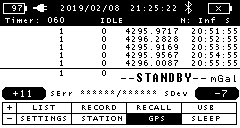
\includegraphics[width=0.49\textwidth]{figures/the_gps_screen_1}
  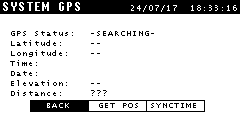
\includegraphics[width=0.49\textwidth]{figures/the_gps_screen_2}
  \caption{Экран GPS}
  \label{fig:the_gps_screen_2}
\end{figure}

Состояние блока GPS будет определено как <<SEARCHING>> (Поиск). После
обнаружения достаточного количества спутников, поля Latitude (Широта), Longitude
(Долгота), Time (Время), Date (Дата), Elevation (Высота над у/моря) и Distance
(Расстояние) заполняются автоматически. Параметр Distance (в метрах)~-- это
расстояние между текущими координатами GPS и координатами пункта наблюдения.

\begin{figure}[h]
  \centering
  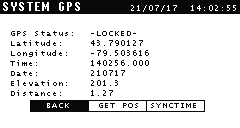
\includegraphics[width=0.49\textwidth]{figures/the_gps_active_screen}
  \caption{Экран активного блока GPS}
  \label{fig:the_gps_active_screen}
\end{figure}

Вы можете обновить широту, долготу и высоту над у/м для вашего текущего пункта
наблюдения, наведя курсор на пункт \textbf{GET POS}, и нажав кнопку
\textbf{Enter}. На дисплее появится следующее экранное изображение:

\begin{figure}[h]
  \centering
  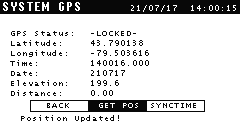
\includegraphics[width=0.49\textwidth]{figures/the_gps_screen_with_locked_positions}
  \caption{Экран GPS с <<захваченными>> координатами}
  \label{fig:the_gps_screen_with_locked_positions}
\end{figure}

Теперь широта, долгота и высота над у/м для вашего текущего пункта наблюдения
обновлены согласно показаниям GPS. Вы можете перейти к экранному изображению
Station для повторной проверки.

\section[Выполнение измерений]{Выполнение измерения при помощи \cg{}}

\subsection[Установка на штатив]{Установка \cg{} на штатив}

Процесс установки прибора \cg{} на штатив показан ниже.

\begin{figure}[h]
  \centering
  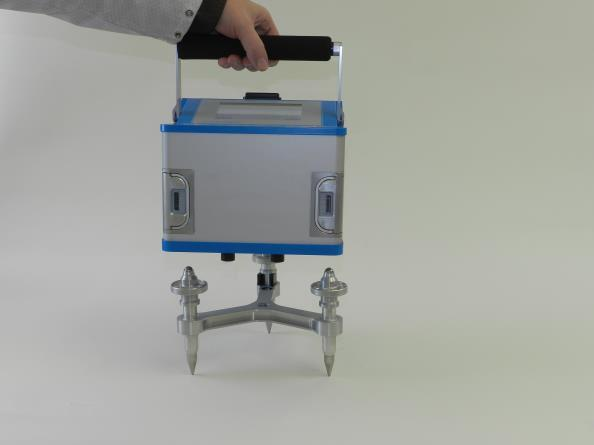
\includegraphics[width=0.49\textwidth]{figures/placing_the_cg6_autograv_on_its_tripod}
  \caption{Установка \cg{} на штатив}
  \label{fig:placing_the_cg6_autograv_on_its_tripod}
\end{figure}

\subsection[Горизонтирование прибора]{Горизонтирование прибора \cg{}}
\label{subsec:leveling_the_cg6_autograv}

Прибор \cg{} предоставляет два типа данных, которые могут быть использованы для
его горизонтирования. Первый тип~- это цифровые показания уровня по осям X и Y,
отображаемые в угловых секундах. Второй тип~-- это две стрелки горизонтирования,
указывающие направление, в котором нужно вращать регулировочные винты штатив 
для горизонтирования прибора в горизонтальной плоскости.

Если прибор устанавливается на штатив в первый раз, стрелки уровня будут, скорее
всего, красными или оранжевыми, в зависимости от того, насколько <<далеко>>
прибор находится от выровненного состояния. Чтобы выровнять прибор, вращайте
регулировочные рукоятки на штатив в указываемом стрелками направлении, пока цвет
стрелок не сменится на зелёный. Пользователь может следить за числовыми уровнями
на экране, чтобы оценить, на какой угол нужно повернуть регулировочные рукоятки
для горизонтирования прибора.

В зависимости от требований конкретной съёмки, пользователь может выбрать
допустимый интервал (интервал, в котором стрелки горизонтирования имеют зелёный
цвет) для корректировки уровня на экранном изображении меню, как описано в
разделе \nameref{subsec:adjusting_the_level_window} на
странице~\pageref{subsec:adjusting_the_level_window}.

Величина интервала уровня~-- это порог, ниже которого цвет стрелок
горизонтирования становится зелёным. Например, если интервал уровня задан равным
10 угловых секунд, тогда в случае, когда величина угла наклона одной из осей не
выходит за пределы \textpm{}10 угловых секунд, соответствующая этой оси стрелка
горизонтирования имеет зелёный цвет.


\begin{figure}[h]
  \centering
  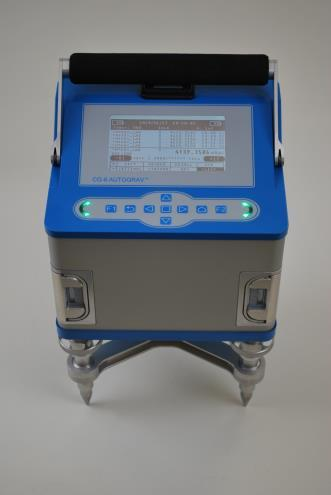
\includegraphics[width=0.49\textwidth]{figures/leveling_arrows}
  \caption{Стрелки горизонтирования}
  \label{fig:leveling_arrows}
\end{figure}

\warningbox{
  Сначала нужно произвести горизонтирование по оси Y, а затем~-- по оси~X.
}

\subsection{Выполнение измерения}

На главном экранном изображении наведите курсор на пункт \textbf{RECORD} и
нажмите кнопку \textbf{Enter}. В верхней части экранного изображения появится
слово \textbf{RECORDING}, как показано на
рисунках~\ref{fig:cg6_autograv_main_screen_idle_mode} и
\ref{fig:cg6_autograv_main_screen_recording_mode}.

\infobox{
  Самый быстрый и простой способ переместить курсор на кнопку записи с любого
  экрана~-- нажать кнопку \textbf{Home}
}


\infobox{
  Если задать короткую задержку записи (обычно 5 секунд), то слабое возмущение,
  вызванное нажатием кнопки Enter, успеет рассеяться до того, как начнётся
  регистрация данных.
}

\infobox{
  Продолжительность измерения~-- это количество циклов * длина цикла измерения.
  Если это ещё не было настроено, обратитесь к разделам
  \nameref{subsec:adjusting_the_number_of_cycles} и
  \nameref{subsec:adjusting_the_measurement_cycle_length} на страницах
  \ref{subsec:adjusting_the_number_of_cycles} и
  \ref{subsec:adjusting_the_measurement_cycle_length}.
}

\section{Просмотр данных}

Вы можете вызвать для просмотра ранее записанные данные под текущим названием
съёмки. Они будут появляться последовательно, друг за другом.

На главном экранном изображении наведите курсор на пункт \textbf{RECALL}
(изображение внизу слева) и нажмите кнопку \textbf{Enter}. Откроется экран,
показанный справа:

\begin{figure}[h]
  \centering
  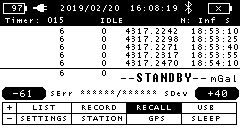
\includegraphics[width=0.49\textwidth]{figures/the_data_recall_screen_1}
  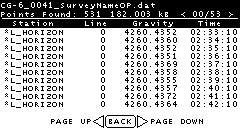
\includegraphics[width=0.49\textwidth]{figures/the_data_recall_screen_2}
  \caption{Экран просмотра данных}
  \label{fig:the_data_recall_screen}
\end{figure}

Для того, чтобы обратиться к данным под другим названием съёмки, перейдите к
\textbf{SETTINGS/SURVEY} и введите название съёмки, под которым вы хотели бы
просматривать данные. Примите изменение и вернитесь в экранное изображение
\textbf{RECALL}~-- вы увидите зарегистрированные данные под этим названием
съёмки.  Если введённое вами название съёмки никогда не использовалось, вы
увидите пустой список.

\begin{figure}[h]
  \centering
  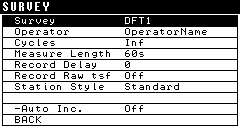
\includegraphics[width=0.49\textwidth]{figures/recalling_data_under_a_different_survey_name_1}
  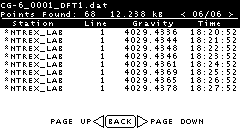
\includegraphics[width=0.49\textwidth]{figures/recalling_data_under_a_different_survey_name_2}
  \caption{Вызов и просмотр данных под другим именем съемки}
  \label{fig:recalling_data_under_a_different_survey_name}
\end{figure}

Чтобы выйти из этого экранного изображения, нажмите кнопку \textbf{Enter}.

\infobox{
  Максимальное число показаний $N_{\max}$, которые вы можете вызвать для
  просмотра, составляет примерно 500. Если полное число показаний в съёмке
  превышает этот лимит, тогда для просмотра будут доступные последние $N_{\max}$
  показаний.
}

\subsection{Извлечение данных}
\label{subsec:taking_a_measurement}

Подключите внешний USB-кабель (номер по каталогу 128370053) к USB-порту на вашем
\cg{} и любому разъёму UBS на вашем ноутбуке или планшете.

\begin{figure}[h]
  \centering
  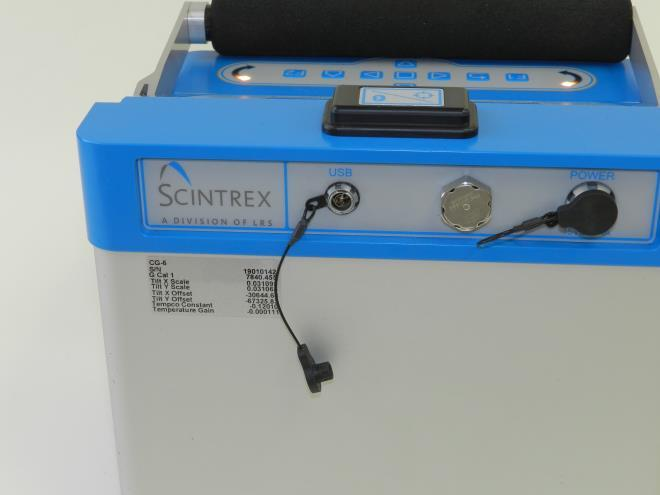
\includegraphics[width=0.49\textwidth]{figures/the_cg6_autograv_usb_port}
  \caption{Порт USB на приборе \cg{}}
  \label{fig:the_cg6_autograv_usb_port}
\end{figure}

Для доступа к режиму USB зайдите в главное экранное изображение и наведите
курсор на пункт \textbf{USB} (изображение внизу слева), после чего нажмите
кнопку \textbf{Enter}.  Откроется экран, показанный справа:

\begin{figure}[h]
  \centering
  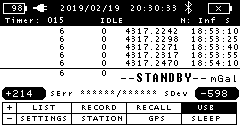
\includegraphics[width=0.49\textwidth]{figures/the_usb_screen_1}
  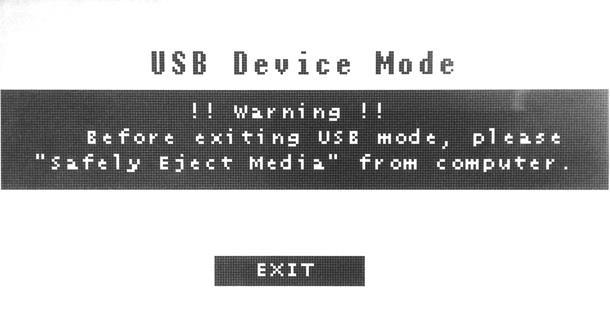
\includegraphics[width=0.49\textwidth]{figures/the_usb_screen_2}
  \caption{Экран USB}
  \label{fig:the_usb_screen}
\end{figure}

\warningbox{
  Прибор \cg{} должен находиться в нерабочем режиме, т.~е., прежде чем режим
  устройства USB, необходимо остановить регистрацию данных.
}

Ваш \cg{} появится на вашем компьютере как запоминающее устройство, как показано
ниже. Вы можете легко переносить файлы на свой компьютер, как с USB-накопителя.

\begin{figure}[h]
  \centering
  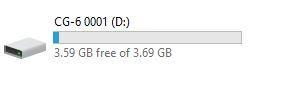
\includegraphics[width=0.49\textwidth]{figures/the_cg6_autograv_as_a_mass_storage_device_on_your_computer}
  \caption{\cg{} как запоминающее устройство на компьютере}
  \label{fig:the_cg6_autograv_as_a_mass_storage_device_on_your_computer}
\end{figure}

Файловая структура прибора \cg{} показана на схеме ниже.


\begin{figure}[h]
  \centering
  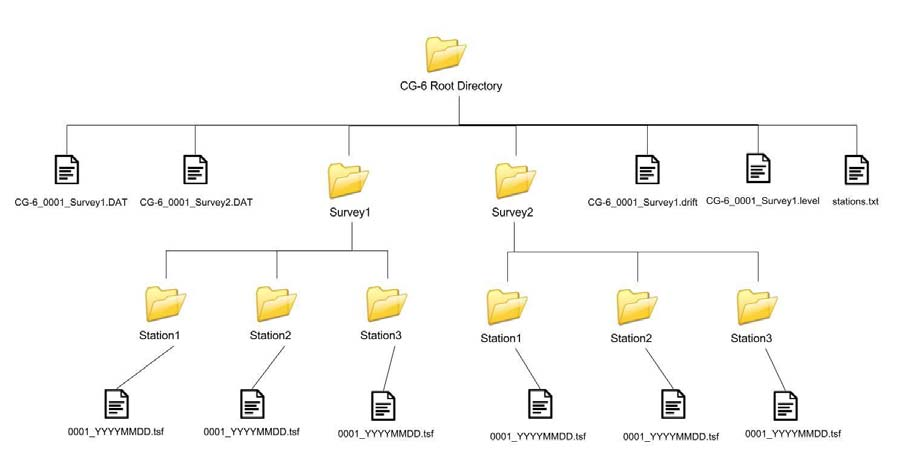
\includegraphics[width=\textwidth]{figures/file_structure_of_a_cg6_autograv}
  \caption{Файловая структура прибора \cg{}}
  \label{fig:file_structure_of_a_cg6_autograv}
\end{figure}

\subsection{Filtered Data File (.DAT)}

В файле фильтрованных данных сохраняются фильтрованные гравиметрические
показания (стандартное отклонение, уровни X/Y, температура датчика, и т.~д.) на
частоте, задаваемой выбранной вами длительностью цикла измерения (30~с, 60~с или
120~с).

После того, как начнётся запись данных, каждый раз при достижении заданной
длительности цикла измерения, в файл фильтрованных данных будет записываться
новая строка с показаниями.

Файл фильтрованных данных сохраняется в корневой директории вашего прибора
\cg{} под именем:

\path{\cg{}-6_XXXX_SurveyName.DAT}

где XXXX – это последние 4 цифры серийного номера измерительного прибора.

На рисунке~\ref{fig:sample_filtered_data_file_from_a_cg6_autograv} приведён
пример файла фильтрованных данных.

\begin{figure}[h]
  \centering
  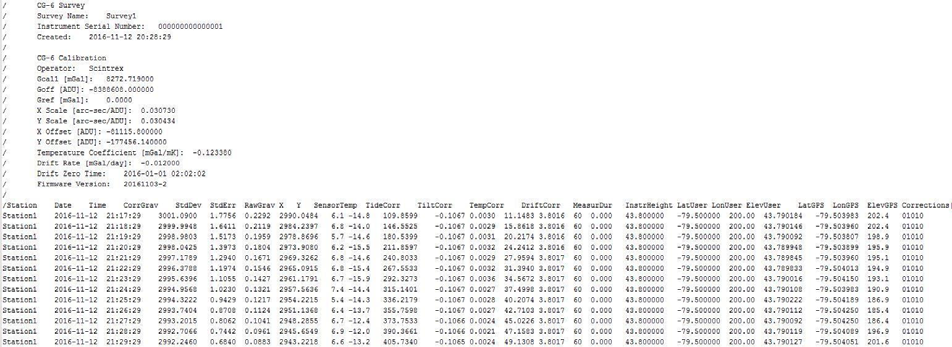
\includegraphics[width=\textwidth]{figures/sample_filtered_data_file_from_a_cg6_autograv}
  \caption{Пример файла фильтрованных данных \cg{}}
  \label{fig:sample_filtered_data_file_from_a_cg6_autograv}
\end{figure}

\subsection{Файл исходных данных TSF (.tsf)}

Файл исходных данных tsf~-- это файл, в котором сохраняются первичные
показания в процессе измерения. В каждой строке файла содержится следующее:
\begin{itemize}
  \item метка времени

  \item 10 первичных гравиметрических показаний (блок ADC)

  \item первичные показания уровня по осям X и Y (блок ADC)

  \item первичное показание температуры (блок ADC)

  \item поправка на земные приливы (мГал)

  \item бит состояния
\end{itemize}

Если активизирована функция Record Raw tsf, новая строка с показаниями будет
добавляться к файлу через каждую секунду в процессе регистрации данных.

Файлы исходных данных tsf систематизируются по съёмке, пункту наблюдения и
дате. Ниже показан путь доступа к файлу.

\path{\SurveyName\StationName\XXXX_YYYYMMDD.tsf}

Прибор CG-6 автоматически создаёт новый первичный файл tsf при выборе новой
съёмки или пункта наблюдения, или при прохождении часами полночи во время
регистрации данных.

Ниже показан пример первичного файла tsf.

\begin{figure}[h]
  \centering
  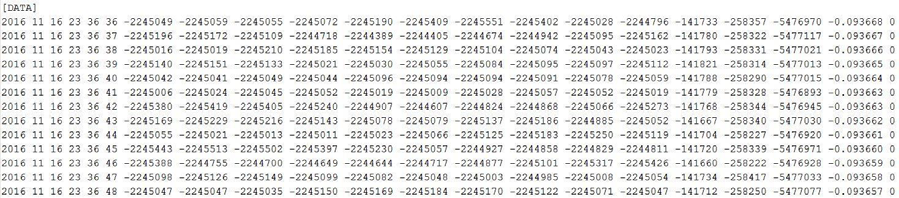
\includegraphics[width=\textwidth]{figures/sample_raw_tsf_file_from_a_cg6_autograv}
  \caption{Пример первичного файла TSF \cg{}}
  \label{fig:sample_raw_tsf_file_from_a_cg6_autograv}
\end{figure}

\subsection{Файл калибровки дрейфа (.drift) и калибровки наклона (.level)}

Файл калибровки дрейфа записывается во время проверки калибровки дрейфа, а файл
калибровки наклона~-- во время проверки калибровки наклона. Оба эти файла имеют
тот же формат, что и файл фильтрованных данных (.DAT), и их можно найти в
корневой директории прибора CG-6. Они имеют следующие файловые имена.

\path{\cg{}-6_XXXX_SurveyName.drift}

\path{\cg{}-6_XXXX_SurveyName.level}

\begin{figure}[H]
  \centering
  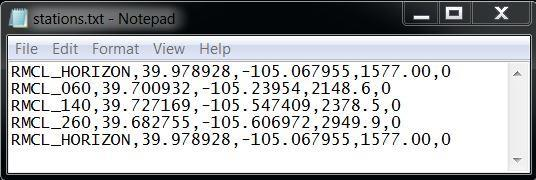
\includegraphics[width=0.8\textwidth]{figures/sample_pre-set_stations_file_from_a_cg6_autograv}
  \caption{Пример файла заранее определённых пунктов \cg{}}
  \label{fig:sample_pre-set_stations_file_from_a_cg6_autograv}
\end{figure}

\subsection{Файл заранее определённых пунктов наблюдения (stations.txt)}

В этом файле хранится список заранее определённых пунктов наблюдения. В
процессе редактирования этого файла вы можете добавлять, удалять или
изменять информацию, касающуюся заранее определённых пунктов наблюдения.
Обратитесь к разделу \nameref{sec:setting_up_the_pre-set_list_of_stations} в
конце главы~\ref{chap:setting_up_your_cg6_autograv}.

